\documentclass[
    iict, % Saisir le nom de l'institut rattaché
    il, % Saisir le nom de l'orientation
    %confidential, % Décommentez si le travail est confidentiel
]{heig-tb}

\usepackage{titlesec}

\titleformat{\chapter}[display]
  {\normalfont\bfseries}{}{0pt}{\Huge}


\usepackage[nooldvoltagedirection,european,americaninductors]{circuitikz}
\usepackage{hyperref}
\usepackage{fancyhdr}
\usepackage{lastpage}

%\signature{mbernasconi.svg} TODO

\makenomenclature
\makenoidxglossaries
\makeindex

\addbibresource{bibliography.bib}

\usepackage{etoolbox}
\renewcommand\nomgroup[1]{%
  \item[\bfseries
  \ifstrequal{#1}{A}{Constantes physiques}{%
  \ifstrequal{#1}{B}{Groupes}{%
  \ifstrequal{#1}{C}{Autres Symboles}{}}}%
]}

\newcommand{\nomunit}[1]{%
\renewcommand{\nomentryend}{\hspace*{\fill}#1}}

\nomenclature[A, 02]{\(c\)}{\href{https://physics.nist.gov/cgi-bin/cuu/Value?c}
{Vitesse de la lumière dans le vide}
\nomunit{\SI{299792458}{\meter\per\second}}}

\nomenclature[A, 03]{\(h\)}{\href{https://physics.nist.gov/cgi-bin/cuu/Value?h}
{Constante de Planck}
\nomunit{\SI[group-digits=false]{6.62607015e-34}{\joule\per\hertz}}}

\nomenclature[A, 01]{\(G\)}{\href{https://physics.nist.gov/cgi-bin/cuu/Value?bg}
{Constante de gravitation universelle}
\nomunit{\SI[group-digits=false]{6.67430e-11}{\meter\cubed\per\kilogram\per\second\squared}}}

\nomenclature[B, 03]{\(\mathbb{R}\)}{Nombres réels}
\nomenclature[B, 02]{\(\mathbb{C}\)}{Nombres complexes}
\nomenclature[B, 01]{\(\mathbb{H}\)}{Quaternions}

\nomenclature[C]{\(V\)}{Volume constant}
\nomenclature[C]{\(\rho\)}{Indice de frottement sec}

\newacronym{gcd}{GCD}{Plus grand diviseur commun}
\newacronym{lcm}{LCM}{Plus petit multiple commun}
\newacronym{uon}{UON}{Unified Object Notation}
\newacronym{antlr}{ANTLR}{Unified Object Notation}
\newacronym{ebnf}{EBNF}{Extended Backus–Naur Form}

\newglossaryentry{heig-vd}{
    name=HEIG-VD,
    description={Haute École d'Ingénierie et de Gestion du canton de Vaud}
}
\newglossaryentry{hes-so}{
    name=HES-SO,
    description={Haute École Supérieure de Suisse Occidentale}
}
\newglossaryentry{latex}{
    name=latex,
    description={Un langage et un système de composition de documents}
}
\newglossaryentry{maths}{
    name=mathematics,
    description={Les mathematiques sont ce que les mathématiciens fonts}
}
\newglossaryentry{token}{
    name=token,
    description={C'est un segment de texte avec un type associé}
}
\newglossaryentry{grammaire}{
    name=grammaire,
    description={un fichier décrivant formellement un langage}
}
% Auteur du document (étudiant-e) en projet de Bachelor
\author{Vitor Vaz Afonso}

% Activer l'option pour l'accord du féminin dans le texte
\genre{male}

% Titre de votre travail de Bachelor
\title{Support du langage UON sous VS Code}

% Le sous titre est optionnel
\subtitle{Travail de Bachelor}

% Nom du professeur responsable
\teacher {Prof. Y. Chevallier (HEIG-VD)}

% Mettre à jour avec la date de rendu du travail
\date{\today}

% Numéro de TB
\thesis{7212}



\surroundwithmdframed{minted}

%% Début du document
\begin{document}
\selectlanguage{french}
\maketitle
\frontmatter
\clearemptydoublepage

%% Requis par les dispositions générales des travaux de Bachelor
\preamble
\let\cleardoublepage\clearpage
\authentification
\let\cleardoublepage\clearpage

%% Résumé / Version abbrégée
\begin{abstract}
    % Francais

% • le contexte,
En 2018, le professeur Yves Chevallier a imaginé un nouveau format de sérialisation proche de YAML et JSON nommé \Gls{uon}.
UON vise à rassembler toutes les caractéristiques utiles des formats de sérialisation les plus utilisés sur internet (XML, YAML et JSON),
en un seul format qui les englobe. Cela dans le but de le rendre adapté à la communication \Gls{m2m} pour des dispositifs embarqués de faibles puissances, jusqu'aux plateformes haut de gamme basées sur le cloud.

% • la problématique,
Ce Travail de Bachelor a pour objectif de permettre l'utilisation du langage UON dans l'éditeur de code VS Code, en créant une extension disponible depuis le Marketplace de Visual Studio Code.
Cette extension doit fournir à l'utilisateur, le support de langage permettant une meilleure rédaction d'un fichier UON.

Le support est fourni sur une implémentation de la grammaire issue de la spécification UON.
L'API de VS Code est directement contactée pour implémenter les fonctionnalités.
ANTLR est le générateur de parser qui a été choisi.
Le moteur de complétion antlr4-c3 est utilisé comme source principale des suggestions pour l'auto-complétion.

Au terme de ce projet, les points attendus du cahier des charges ont été effectués. Il s'agit de :
\begin{itemize}
    \item Disposer d'une grammaire du langage UON utilisable
    \item Implémenter une intégration continue
    \item Implémenter une coloration syntaxique
    \item Implémenter de l'auto-complétion
    \item Implémenter une outline view
    \item Implémenter l'affichage des informations au survol de la souris (Hover Information)
    \item Implémenter un Linter simple pour signaler des erreurs
\end{itemize}

% • perspectives et recommandations
Les perspectives concernant ce sujet sont vastes, mais des améliorations possibles à ce projet sont les suivants :
\begin{itemize}
    \item Implémenter les points du CDC dans la partie "si le temps le permet".
    \item Utiliser un langage server au lieu de l'API VS Code.
    \item Continuer à améliorer la grammaire et adapter les fonctionnalités en conséquence.
\end{itemize}
\end{abstract}

%% Sommaire et tables
\listoffigures
\addcontentsline{toc}{chapter}{\listfigurename}
\listoflistings
\addcontentsline{toc}{chapter}{Liste des codes sources}

\tableofcontents

\printnomenclature
\clearemptydoublepage
\pagenumbering{arabic}

\pagestyle{fancy}
\fancyhf{}
\renewcommand\headrulewidth{1pt}

\fancyhead[R]{Support du langage UON}
\fancyhead[L]{\itshape\nouppercase{\leftmark}}

\renewcommand{\chaptermark}[1]{\markboth{\MakeUppercase{#1}}{}}

\renewcommand\footrulewidth{1pt}

\fancypagestyle{plain}{%
    \fancyfoot[R]{Page \thepage/\pageref{LastPage}}
}
\fancyfoot[R]{Page \thepage/\pageref{LastPage}}

\renewcommand{\headrulewidth}{0.4pt}
\renewcommand{\footrulewidth}{0.4pt}


%% Contenu
\mainmatter
\chapter{Introduction}
Ce projet de Bachelor consiste à fournir du support pour le nouveau langage de sérialisation UON, sous VsCode. Ce projet se veut expérimental. C'est-à-dire qu'aucun cadre précis sur sa réalisation n'a été établi et que les approches choisis sont libres tant qu'elles respectent le cahier des charges.
Dans les chapitres suivants, nous allons voir ce qui est fourni par VsCode pour élaborer et déployer une extension.
Les éléments à prendre en compte pour pouvoir fournir du support pour un langage.
Les aspects du langage UON à considérer dans le cadre de ce projet.
Et présenterons en détail l'implémentation d'une extension ainsi que ses fonctionnalités. Puis détaillerons les tests effectués.

\let\cleardoublepage\clearpage

\chapter{Cahier des charges}
Voici ci-dessous un résumé du cahier des charges :

\textbf{Extension}
\begin{itemize}
    \item Code source publié sur Github
    \item Fournir une intégration continue
    \item Déployer l'extension sur le marketplace
\end{itemize}

\textbf{Fonctionnalités à implémenter}
\begin{itemize}
    \item Syntax highligting
    \item Auto-complétion
    \item Document Outlining
    \item Hover Information
\end{itemize}

\textbf{Si le temps le permet}
\begin{itemize}
    \item Lint
    \item Formatter
    \item Converter
\end{itemize}

\vspace{\parskip}

Ce projet se focalise uniquement sur l'éditeur de code VScode.

Une extension peut être écrite en Typescript ou en Javascript.
Nous choisirons le Typescript car Vscode recommande ce langage.

Concernant les fonctionnalités à implémenter. Il n'y avait pas de contraintes de choix.
Nous avons donc séléctionner les fonctionnalités attendues en choisissant celles paraissant utiles à avoir dans un premier temps et en prenant en considération la contrainte de temps.

\chapter{Pré-étude}

\section{VScode}
Visual Studio Code (ou VScode) est un éditeur de code qui est pensé pour être extensible (De L'UI à l'expérience utilisateur).
Presque tout peut être customisé et améliorer à travers de \href{https://code.visualstudio.com/api/extension-capabilities/overview}{L'Extension API}.

L'Extension API nous permet donc gérér un certain nombre de choses.
On se focalisera sur le theming , les fonctionnalités de langages, la publication de l'extension et les tests.

VScode fourni pleins de documentations détaillées sur plein de sujets, guides, ainsi que des examples de codes.
Il s'agit donc évidemment de la source principales des explications données dans ce document concernant ce qui touche à cette éditeur.

\subsection{Extension Anatomy}
Il y a 3 concepts crucials à comprendre pour réaliser une extension.

\begin{itemize}
    \item \textbf{\href{https://code.visualstudio.com/api/references/activation-events}{Activation Events}}: Des événements à partir desquels l'extension devient active.
    \item \textbf{\href{https://code.visualstudio.com/api/references/contribution-points}{Contribution Points}}: Des déclarations statiques qui sont faitent dans l'Extension Manifest "package.json" pour étendre l'extension. Il s'agit d'un ensemble de déclarations JSON faites au travers du champ "contributes".
    \item \textbf{\href{https://code.visualstudio.com/api/references/vscode-api}{VS Code API}}: Un ensemble d'API JavaScript que nous pouvons invoquer dans le code.
\end{itemize}

En général, l'extension est une combinaison de plusieurs Conntribution Point et de VS code API pour étendre les fonctionnalité de VSCode.

\subsubsection{Extension File Structure}\label{Extension File Structure}
La structure d'une extension est la suivante :
\begin{lstlisting}
    .
    ├── .vscode
    │   ├── launch.json     // Config for launching and debugging the extension
    │   └── tasks.json      // Config for build task that compiles TypeScript
    ├── .gitignore          // Ignore build output and node_modules
    ├── README.md           // Readable description of your extension's functionality
    ├── src
    │   └── extension.ts    // Extension source code
    ├── package.json        // Extension manifest
    ├── tsconfig.json       // TypeScript configuration
\end{lstlisting}

\textbf{Extension Manifest} :
Chaque extension doit contenir un fichier "package.json". En plus des champs propre à Node.js, on peut spécifier des scripts, dépendances de dévelopement et des champs spécifiques à Vscode.

\textbf{Extension Entry File} :
Il s'agit du fichier prinicipale de l'extension (Extension.js).
De base il contient 2 fonctions : "activate" et "deactivate".
La fonction activate est executé à l'activation de notre extension par un Activation Event. On définira ici le code à exécuter.
La fonction deactivate  ext exécuté lorsque l'application devient innactive. Et sert principalement à nettoyer le code avant la désactivation de l'extension

\textbf{Remarque} : Le niveau de customisation est assez élevé. La seul limitation souvent indiquée et qu'il n'est pas possible d'accéder au DOM de l'éditeur.

Nous avons donc vu les briques de bases pour la conception d'une extension. Cette base est suffisante pour nous dans un premier temps.
Comme ce rapport n'a pas pour vocation d'expliquer tout ce qui est possible de faire dans une extension. Si vous souhaitez vous renseigner d'avantages sur ce sujet, vous pouvez le faire \href{https://code.visualstudio.com/api}{ici}.

La même remarque concerne aussi les fonctionnalités général de l'éditeur VScode. Pour plus de détail, consulter \href{https://code.visualstudio.com/docs}{la documentation officielle}.

\subsection{Support de langage}
VsCode fournit la possibilité d'ajouter du support pour un nouveau langage de programmation au travers d'implémentation de fonctionnalités. Ces fonctionnalités peuvent être classées en 2 catégories :

\section{Declarative language features}
Elles ajoutent un support d'édition de texte de base pour un langage de programmation.
Par exemple, les éléments suivants :

\begin{itemize}
    \item Syntax highlighting
    \item Snippet completion
    \item Bracket matching
    \item Bracket autoclosing
    \item Bracket autosurrounding
    \item Comment toggling
    \item Auto indentation
    \item Folding (by markers)
\end{itemize}

Il s'agit de fonctionnalités implémentées à l'aide de fichier de configuration.

Puis, elles doivent être enregistrées comme Contribute Point.

\section{Programmatic language features}
Il s'agit de fonctionnalité plus riche donc plus complexe à mettre en place (p.ex : "Hovers", "Go to Definition", "diagnostic errors", "IntelliSense" \space et "CodeLens".
Il y a 2 approches pour les implémenter que nous allons voir ci-dessous.

\subsection{VsCode API (Direct implementation)}
La première solution est d'utiliser l'api \href{https://code.visualstudio.com/api/references/vscode-api#languages}{vscode.languages.*} qui expose des interfaces
permettant de réaliser directement les fonctionnalités.

Elle vont nous permettre de nous s'inscires à des providers. L'éditeur de code fera ensuite les requêtes à ces providers lorsque cela sera nécessaire.

\subsection{Langage server}
La seconde solution est de fournir nous-mêmes ces méthodes en respectant \href{https://microsoft.github.io/language-server-protocol/specifications/lsp/3.17/specification/}{la spécifiation LSP} au travers d'un langage serveur.
Les avantages souvent mentionnés ce cette approche et que le langage server peut être écrit avec le langage que l'on souhaite et
que cela permet aussi à d'autres éditeurs de texte compatibles avec le langage server d'utiliser ses fonctionnalités sans devoir les implémenter de nouveau.

Mais comme points négatifs cette approche est plus complexe à implémenter et dans notre cas n'est pas un choix primordial.

Pour être utiliser sur VSCode, un langage server à 2 partis :
\begin{itemize}
    \item \textbf{Un client} : C'est une extension écrite en Javascript ou Typescript qui à accès à tous les endpoints de VScode
    \item \textbf{Langage server} : Un outil d'analyse linguistique fonctionnant dans un processus séparé lancé
\end{itemize}

Le client et le serveur communiquent à l'aide du protocole LSP (pour "language server") dès que des informations riches devraient être fournies à l'éditeur.
Le langage server devrait donc ensuite pouvoir "consommer" un parser pour traiter les fonctionnalités. C'est-à-dire être capable d'analyser un AST et de fournir une réponse adéquate.
L'implémentation d'un tel serveur peut être libre, mais des implémentations existent déjà. Telle que "LSP4" implémenté en Java ou  "Vscode-languageserver-node" implémenté en Typescript qui n'est pas exclusivement réservé à VsCode comme son nom pourrait l'indiquer.
On remarque donc avec cette approche que 2 composantes existent (Le client et le serveur)
Un langage server peut être utilisé sur d'autre éditeur compatible. Mais le client devra être implémenté de nouveau.

\subsection{API vs LSP}\label{api vs lsp}

Ce schéma ci-dessus montre la correspondance des méthodes entre la première et seconde approche.
Cette liste est non exhaustive mais permet de montrer que les 2 approches sont relativement bien supporté.

\begin{figure}[!ht]
    \begin{center}
        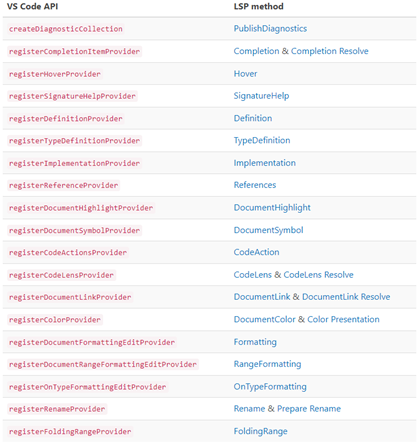
\includegraphics[width=10cm]{assets/figures/api-vscode.png}
    \end{center}
    \caption[API vs LSP]{\label{api vs lsp} VS Code API vs LSP method}
\end{figure}

\subsection{Parser}
Pour fournir des fonctionnalités de langue, une approche souvent pratiqué et l'utilisation d'un parser.
Car les fonctionnalité se baseront sur L'AST qu'il générera.

Cependant dans le cadre de son utilisation dans un éditeur/IDE, il devrait être "fault tolerant". Le parseur doit pouvoir générér un AST (abstract syntax tree) qui à du sens depuis du code incomplet.

Il ne devrait pas s'arrêter dès la première erreur. Car la plupart du temps, le code dans l'éditeur est incomplet et syntaxiquement incorrect.
Et les développeurs s'attendent tout de même à ce que la complétion automatique et et d'autres fonctions de langue fonctionnent.

\subsection{Grammaire}
Il faudra aussi élaborer une grammaire pour le langage de sérialisation UON utilisable par le parser.
Pour faciliter l'étape de l'analyse syntaxique ("Parsing"), cette grammaire pourrait être plus permissive, en particulier concernant les types attendus (Terminaux).
Ainsi si l'utilisateur entre une valeur dont le type attendu est incorrect (par rapport aux spécifications du langage). Nous n'avons pas à traiter ce type d'erreur.

\section{Choix technologiques}
Nous allons mentionner les technologies et approches choisis et expliquer la raison.

\subsection{Direct implementation}
L'implémentation d'un langage serveur n'étant pas une priorité et pour se concentrer sur la réalisation des fonctionnalités, l'approche de contacter directement l'api de VsCode sera choisi.
Si le temps le permet, toute la logique du code concernant les fonctionnalités pourrait être déplacée dans un langage server.

Beaucoup de possibilités existent comme mentionné au point \hyperref[api vs lsp]{API vs LSP}, mais nous utiliserons uniquement les providers suivants :

\begin{itemize}
    \item \textbf{registerCompletionItemProvider} :  Pour afficher des suggestions de complétions
    \item \textbf{registerHoverProvider} : Pour gérer le hover
    \item \textbf{registerDocumentSymbolProvider} : Pour afficher les éléments dans la Outline View
\end{itemize}

\subsection{ANTLR}
\subsubsection{Parser}
Étant donné que ce n'est pas le sujet de notre Travail de Bachelor, je vais m'aider d'outil existant pour extraire le plus possible de complexité concernant ce sujet.
Plein d'outils permettant la génération existe à partir d'une grammaire. Mais allors choisir le générateur de parser d'ANTLR (ANother Tool for Language Recognition) car :

\begin{itemize}
    \item C'est un outil populaire est encore utilisé.
    \item Il est disponible directement en Typescript (\href{https://github.com/tunnelvisionlabs/antlr4ts}{antlr4ts}).
    \item Un moteur de complétion existe avec les parser générés avec antlr. Nous simplifions de grandes étapes pour implémenter l'auto-complétion (\href{https://github.com/mike-lischke/antlr4-c3}{antlr4-c3})
    \item Quelques exemples existent d'implémentation.
    \item La génération est simple. Pour générer un parser (et d'autres fichiers utiles), il suffit d'écrire un fichier contenant une grammaire valide.
\end{itemize}

\textbf{Remarque} :
Comme mentionner au point \hyperref[grammar scope]{Scope de la grammaire}. Mon précesseur avait utilisé Lark pour écrire sa grammaire et générer son Parser pour son travail.
L'implémentation de son parser n'a pas été prévilégié car il aurait été nécessaire de créer l'infrastructure permettant d'utiliser son parser.
Et Antlr semble être un choix plus naturelle dans notre environnement vscode.

\section{UON}
UON est essentiellement un langage de sérialisation qui est un superset de JSON et un superset partiel de YAML.
Il cherche à regrouper les meilleures caractéristiques de ces formats de sérialisation en un seul format.
Il fournit également des fonctionnalités supplémentaires utiles pour augmenter l'interopérabilité entre différents types de dispositifs, valider les données ainsi que pour diminuer le payload.

Nous allons voir ci-dessous un apercu général de ce langage.

\subsection{Pourquoi ?}
Son rôle est d'être utilisé dans l'industrie 4.0. Plus particulièrement dans la communication m2m (machine to machine) ainsi que pour l'IoT (Internet of Things).
Ces communications nécessitent souvent de communiquer entre de petits appareils dont la puissance de calcul est très limitée.
La perspective de disposer d'un protocole de communication applicatif à la fois interopérable et adapté aux échanges à faible puissance est un très apréciable.

\subsection{Communication}
Lorsque deux appareils veulent échanger des informations, ils disposent de deux canaux de communication :
\begin{itemize}
    \item un canal de communication en ligne utilisé pour la transmission des données de contenu (payload). Les données peuvent être représenté sous forme humaine et binaire.
    \item un canal de communication contractuel utilisé pour l'accord sur la description des données (schema).
\end{itemize}

Dans l'image suivante, on a à gauche deux dispositifs : un capteur de température à faible consommation
et une puissante passerelle domotique. Pour réduire la taille du payload, les deux dispositifs peuvent convenir d'un schéma qui décrit le format des données.

\begin{figure}[!ht]
    \begin{center}
        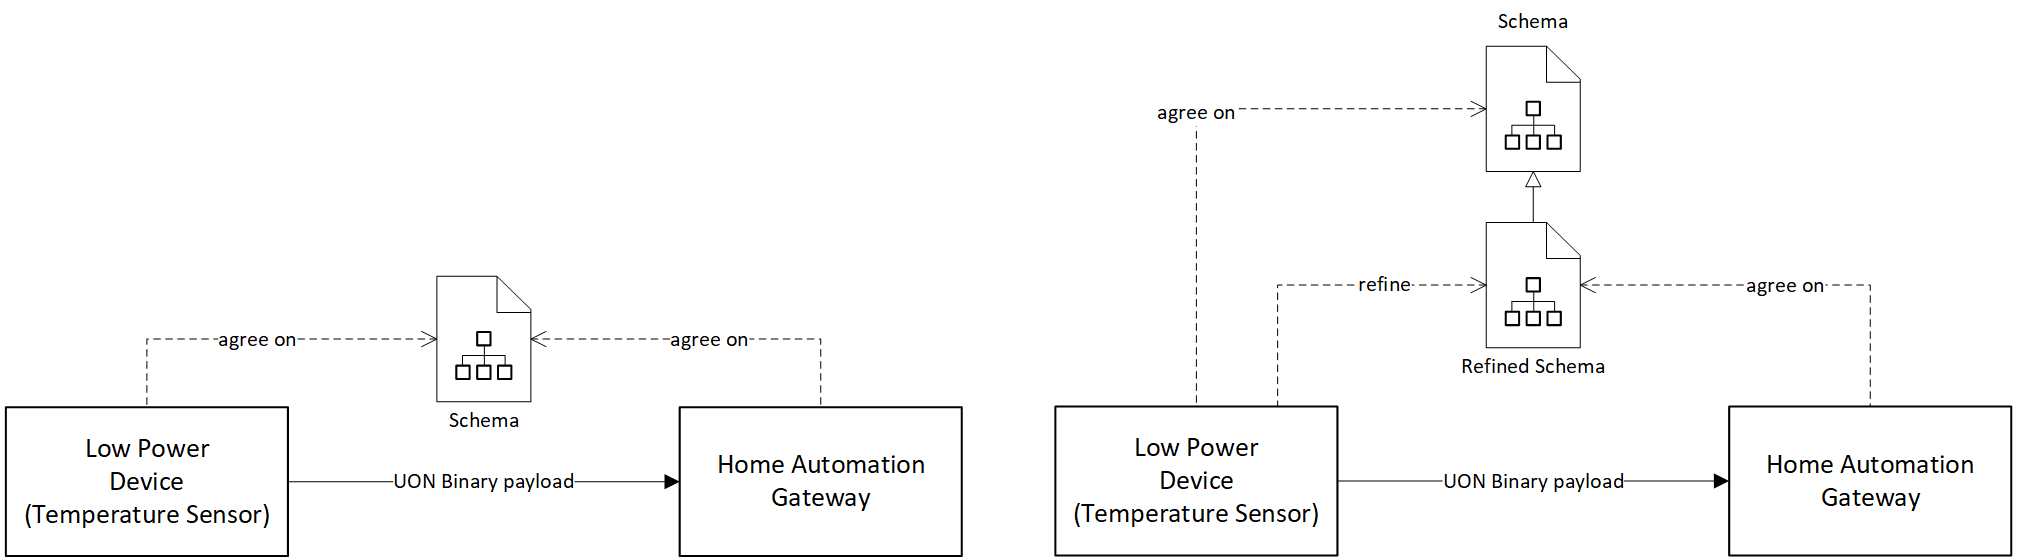
\includegraphics[width=10cm]{assets/figures/data-exchange.png}
    \end{center}
    \caption[UON data exchange]{\label{data-exchange}UON data exchange}
\end{figure}

À droite on affine le schéma. Pour réduire d'avantange les données transmis.
Par exemple en disant que la temperature exprimé avec un nombre et maintenant une valeur non signée de huit bits exprimée en degrés Celsius.

\subsection{Design}
UON est complètement conforme avec JSON et partiellement avec YAML.

UOn peut être classé au travers de 4 niveaux de compléxités :
\begin{itemize}
    \item \textbf{UON:0} est entièrement compatible avec JSON en ce qui concerne le RFC8259
    \item \textbf{UON:1} est partiellement conforme à YAML.
    \item \textbf{UON:2} fournit des propriétés de type, la coercition et les chaînes de caractères multilignes.
    \item \textbf{UON:3} offre des types et des références riches
\end{itemize}

\subsection{Types}
Chaque élément est composé d'un type. Et chacun de ces types peut avoir des propriétés.
3 types de propriétés existent :
\begin{itemize}
    \item \textbf{Presenentation properties} : Elles influencent la présentation d'une valeur.
    \item \textbf{Validation propeties} : Elles sont utilisés pour valider, contraindre et décrire un fichier UON.
    \item \textbf{Application properties} : Elles ne peuvent être lues que depuis UON en utilisant le type !prop. Elles sont accessibles depuis l'application (Python, JavaScript, ...). Elles sont utilisées pour générer un fichier sérialisé (binaire, ou UON), mais elles ne sont jamais explicitement transmises.
\end{itemize}

\subsection{Validation}
Dans de telles communications, la validation des données transmises entre des machines dont la puissance de calcul est très limitée est un atout majeur.
Une des propriétés uniques de UON est l'usage de schéma directement intégré dans le langage.
Le rôle de ce schéma et que les machines se mettent d'accord entre elles sur le format des données à respecter, diminuant ainsi le payload total et s'assurant de la validité des données.

\subsection{Liens}
Si vous souhaitez-vous rensigner d'avantages, la spécification complète du projet se trouve sur cette \href{https://github.com/uon-language/specification/}{page}.
Et le dépôt du projet se trouve \href{https://github.com/uon-language/specification}{ici}.

\chapter{Scope de la grammaire}\label{grammar scope}
Pour pouvoir proposer du support pour un nouveau langage, il est nécessaire de savoir sur quoi celui-ci portera. Il est donc important préciser sur quels éléments du langage (grammaire) nous nous focaliserons.
Nous allons donc partir d'une grammaire la plus minimale possible tout en faisant attention à son extensibilité par la suite.
Cette grammaire se trouve dans le fichier UON.g4.

Elle est une adaptation de la grammaire écrite en Lark par l'ancien élève Stéphane Selim pour son travail de bachelor "Parser for a serialization language UON". Son travail se trouve sur :
\href{https://github.com/uon-language/uon-parser}{https://github.com/uon-language/uon-parser}

Elle sera complétée et améliorée après la mise en place des fonctionnalités attendus et si le temps le permet.

Les fonctionnalités implémentées s'appuieront sur cette grammaire. Ceci dans le but de rester cohérents entre eux.

\textbf{Rappel}
La grammaire actuelle nous permet de définir des maps, séquences dans le format json et yaml. D'ajouter des propriétés à des types et également la possibilité de définir un schéma pour un type custom.

\section{Modification}
\textbf{[TODO]}
\cite{test}

\chapter{Implémentation}
Dans ce chapitre, nous allons explorer les aspects techniques concernant l'implémentation de fonctionnalités. Nous allons voir également plus en détail les outils utilisés ainsi que le déploiement de l'extension sur le marketplace.
Ce travail reflète uniquement mon approche personnelle sur la matière. Et ne devrait pas être considérée comme l'unique manière de procéder.

\section{Code}
Le code de l'implémentation est disponible sur le dépôt public \href{https://github.com/vitorva/vscode-uon}{suivant}.

\textbf{Remarque} : L'implémentation détaillée dans ce rapport pourrait ne plus représenter l'état du dépôt, car ce projet est sujet à évoluer.

\section{Extension}
Nous allons voir maintenant, la procédure pour créer et publier son extension.

\subsection{Génération de l'extension}
VsCode permet de générer un squelette (boilerplate) pour la réalisation d'une extension. Pour ce faire il faut avoir Node.js et Git installés, pour installer Yeoman et VS Code Extension Generator avec la commande :

\begin{lstlisting}[caption={generator-code},label={generator-code}]
npm install -g yo generator-code
\end{lstlisting}

Puis il suffit de saisir la commande :

\begin{lstlisting}
yo code
\end{lstlisting}

et de compléter ce qui est attendu dans le terminal.

\begin{figure}[!ht]
    \begin{center}
        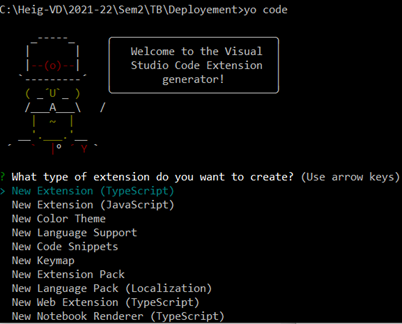
\includegraphics[width=5cm]{assets/figures/yo-code.png}
    \end{center}
    \caption[Yo Code generator]{\label{yo-code}Yo Code generator}
\end{figure}

Cela nous créera l'arborescence mentionné précédement au point \hyperref[Extension File Structure]{Extension File Structure}.

\subsection{Lancement de l'extension en debug}
On peut lancer une nouvelle fenêtre (f5) qui va contenir notre extension.

Par défaut, l'application généré vient avec du code permettant d'afficher le message suivant : "Hello World from [nom de l'extension]" en bas de l'écran. On l'affiche au travers du command pannel (CTRL + SHIFT + P). On peut s'assurer comme cela que l'implémentation de base fonctionne correctement.
On constate donc que l'on peut lancer notre application au travers d'une commande, mais pour notre cas il sera plus intéressant que vscode nous propose les fonctionnalités à l'ouverture d'un fichier. uon.
Pour cela, il faut donc remplacer le code dans le fichier package.json :

\subsection{Déploiement sur le Marketplace}

\textbf{Prérequis} : Posséder un compte Azure.
Il faut récupérer un Personal Access Token , pour ce faire, il faut créer une \href{https://docs.microsoft.com/en-us/azure/devops/organizations/accounts/create-organization?view=azure-devops}{organisation}.
Puis, créer un access token avec ces paramètres :
\begin{figure}[!ht]
    \begin{center}
        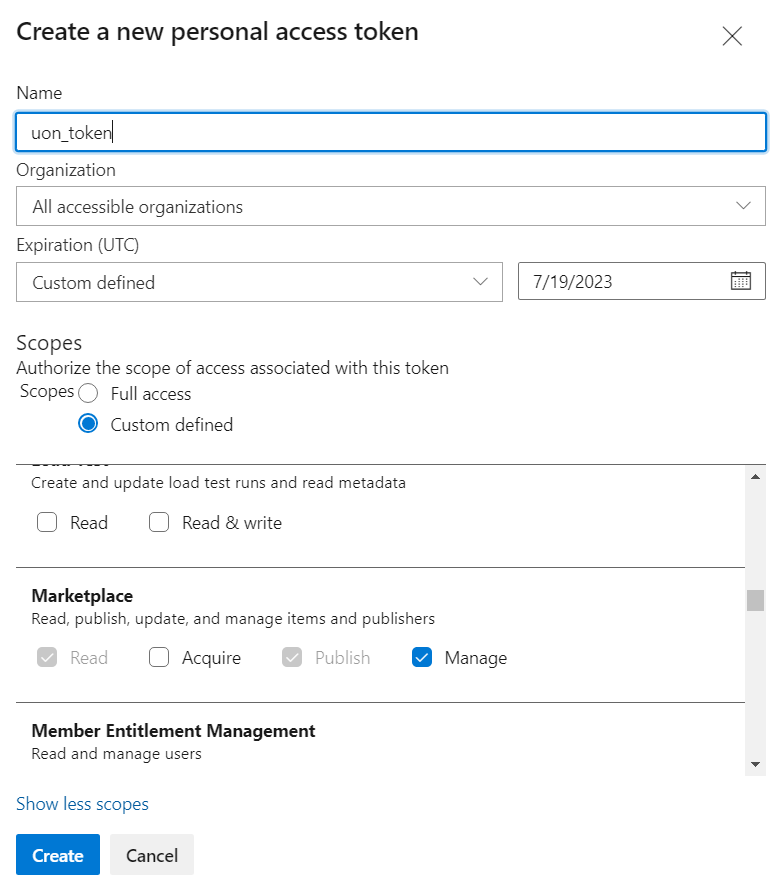
\includegraphics[width=5cm]{assets/figures/access-token.png}
    \end{center}
    \caption[Access Token]{\label{access-token}Access Token}
\end{figure}

Créer un publisher avec le même compte qui a créé l'organisation et le token ci-dessus via la \href{https://marketplace.visualstudio.com/manage/publishers/}{management page}

Ajouter la propriété "publisher" et saisir l'id de celui-ci dans le package.json :

\begin{figure}[!ht]
    \begin{center}
        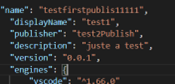
\includegraphics[width=5cm]{assets/figures/json-publisher.png}
    \end{center}
    \caption[Ajout du publisher dans le fichier package.json]{\label{json-publisher} Ajout du publisher dans le fichier package.json}
\end{figure}

Puis saisir dans le terminal : "vsce login [le nom du publisher]"
Puis "Vsce publish" et "accept"

\textbf{Remarque} : Attention au terminal utilisé. Le terminal de node (git.bash) ne propose pas toujours les options de sélections à l'utilisateur. Dans mon cas il était impossible de saisir le PAT et donc une erreur est affichée.
Il est facile en suite de manager l'extension au travers de la page web :
L'extension apparaitra automatiquement dans le marketplace si elle est publié.

\begin{figure}[!ht]
    \begin{center}
        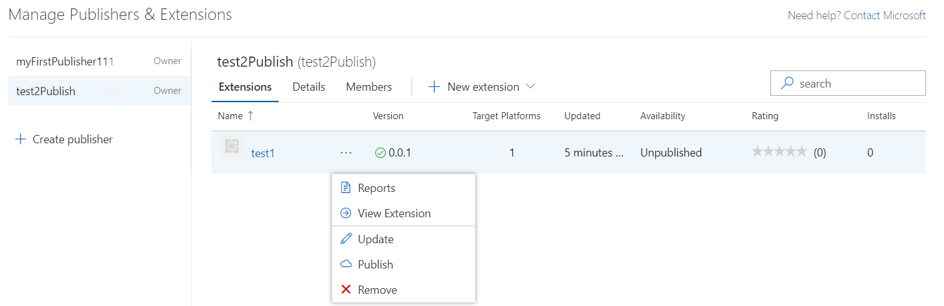
\includegraphics[width=10cm]{assets/figures/manage-publisher.png}
    \end{center}
    \caption[Interface web pour manager l'extension]{\label{manage-publisher} Interface web pour manager l'extension}
\end{figure}


\section{Génération du Parser ANTLR}
\subsubsection{Grammaire}
Le fichier de grammaire doit respecter les points suivants : \textbf{[TODO]}

\textbf{Attention} : Utiliser des majuscules pour une règle, correspond à définir un "Lexer rule" et utiliser des minuscules à un  "Parser rule".

Quand le fichier de grammaire est écrit, il suffit de lancer le code suivant :

\begin{lstlisting}
    antlr4ts UON.g4 -no-listener -no-visitor -o generated -Xexact-output-dir
\end{lstlisting}

Il nous génère les fichiers suivants :
\begin{itemize}
    \item UON.interp
    \item UON.tokens
    \item UONLexer.interp
    \item UONLexer.tokens
    \item UONLexer.ts
    \item UONParser.ts
\end{itemize}

\subsection{Arbre (CST)}
Antlr va génrer un arbre parsé. Plus précisement un CST (concrete syntax tree)
Il contient tous les noeuds de la grammaires. Certains sont superflu pour en tirer un sens

Si on veut un AST, on doit parcouir l'arbre (avec des visiteurs ou listeners) pour en tirer un arbre plus simple.

\begin{figure}[!ht]
    \begin{center}
        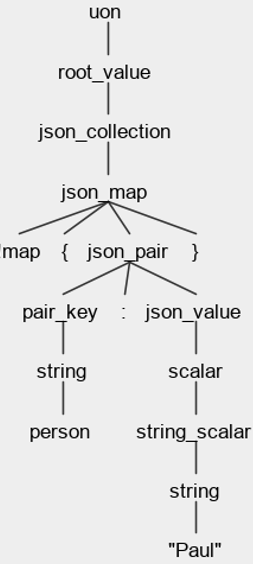
\includegraphics[width=2cm]{assets/figures/tree.png}
    \end{center}
    \caption[UON CST]{\label{uon-tree} UON CST}
\end{figure}

\textbf{[TODO]}

\section{Syntax highlighting}
La coloration syntaxique permet que chaque élément du texte soit affiché dans l'éditeur avec une coloration et un style en fonction de son type.
Il y a 2 composantes principales.
\begin{itemize}
    \item La tokenisation qui consiste à séparer le texte en une liste de token.
    \item La thémisation (Theming) qui permet d'attribuer à un token une couleur et un style.
\end{itemize}

\begin{figure}[!ht]
    \begin{center}
        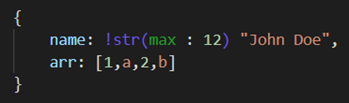
\includegraphics[width=10cm]{assets/figures/basic-uon.png}
    \end{center}
    \caption[code UON]{\label{basic-uon} Exemple basique en UON}
\end{figure}


VS code utilise \href{https://macromates.com/manual/en/language_grammars}{Textmate grammars} comme le moteur de tokénisation de la syntaxe.
Cette grammaire a été inventé par l'éditeur TextMate est a été adopté par de nombreux éditeur et IDE.
Elle contient une liste structurée d'expressions régulière qui permet d'associer un scope à un token.
Nous définissons notre grammaire TextMate dans le fichier "uon.tmLanguage.json" qui  se trouve dans le dossier "syntax" à la racine du projet.
Ce fichier doit être référencé à travers du point de contribution "grammar" dans le package.json.

Le but de ce fichier en plus de permettre la coloration syntaxique, et qu'il permet également de rendre l'éditeur de texte "intelligent" quant au contexte dans lequel se trouve le caret. Cela permet d'avoir des comportements différents selon la situation (ex : Pas de bracket closing dans les commentaires).

\subsection{Scope}
Un scope défini le contexte du token et peut-être considéré comme son type.
TextMate fourni une liste de scope communs que de nombreux thèmes ciblent déjà et recommande de les utiliser. Ceci dans le but de permettre à notre langage d'être supporté le plus possible partout.
Les scopes sont souvent imbriqués et c'est le plus spécifique qui est utilisé pour le choix du thème.
Il est possible d'analyser notre code à l'aide du "Scope Inspector" pour visualiser la hiérarchie des scopes pour un token.

\begin{figure}[!ht]
    \begin{center}
        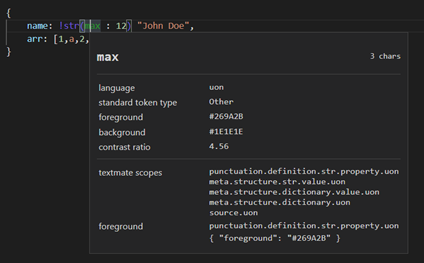
\includegraphics[width=10cm]{assets/figures/scope-inspector.png}
    \end{center}
    \caption[Scope inspector]{\label{basic-uon} Le scope inspector sur un exemple de code en UON}
\end{figure}

La section "textmate scopes" montre la liste des scopes utilisés pour le token qu'on séléctionne. Le scope le plus spécialisé se trouve au sommet.

Cette fonctionnalité n'est pas considérée comme un "programmatic language feature" et donc n'est pas géré par un langage serveur ou depuis l'api de Vscode. Une des raisons évoquées et que ce mécanisme doit être le plus rapide possible. Et que le faire directement depuis le client garantit une latence faible.

\subsection{Stratégie concernant les noms}
Pour respecter au maximum les conventions attendues et s'assurer qu'une coloration automatique soit appliquée. La stratégie suivante a été adoptée : partir depuis un fichier de thème déjà créer (Thème dark par défaut). Et de réutiliser les scopes.

Ce fichier se trouve sur le dépôt \href{https://github.com/microsoft/vscode/blob/main/extensions/theme-defaults/themes/dark_vs.json}{suivant}.
Mais peut être également généré depuis le contrôle panel.

\subsection{Forcer le choix des couleurs}
\begin{figure}[!ht]
    \begin{center}
        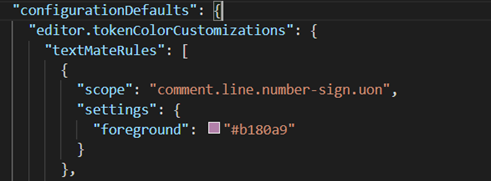
\includegraphics[width=10cm]{assets/figures/manual-settings-color.png}
    \end{center}
    \caption[Choix manuel des couleurs]{\label{manual-settings-color} Choix manuel des couleurs}
\end{figure}

On peut manuellement définir une couleur à un scope dans le fichier package.json.
Cela peut -être intéressant si aucun thème n'est associé de base à un scope.
Il est également possible de créer directement un fichier de thème.

\subsection{Fonctionnement}
\textbf{Exemple simple}

Voici ci-dessous un exemple relativement simple, mais permettant de comprendre le mécanisme général utilisé dans notre fichier uontmLanguage.json :
\begin{lstlisting}
 1  {  scopeName = 'source.untitled';
 2     patterns = (
 3        {  name = 'keyword.control.untitled';
 4           match = '\b(if|while|for|return)\b';
 5        },
 6        {  name = 'string.quoted.double.untitled';
 7           begin = '"';
 8           end = '"';
 9           patterns = (
10              {  name = 'constant.character.escape.untitled';
11                 match = '\\.';
12              }
13           );
14        },
14     );
15  }
\end{lstlisting}

\textbf{"scopeName"} (ligne 1) : Identifiant unique
\textbf{"patterns"} (ligne 2) : C'est un tableau contenant les règles actuelles utilisé pour parser le document. Elles sont appliquées dans l'ordre.
Ces règles peuvent être directement écrites à cet emplacement, mais il est aussi possible de les définir dans le "repository". Puis de les inclure.
\textbf{"repository"} : Un dictionnaire (clé-valeur) de règles.
\textbf{"name"} : Nom du scope.

Contrairement à la première règle qui ne faisait qu'un match, la deuxième définit un début et une fin sur laquelle seront appliquées les règles se trouvant dans le "patterns" suivant (à la ligne 12) . On voit qu'il est donc possible d'imbriquer les règles.

\subsection{Semantic Highlight}

Un point important et qu'il ne faut pas confondre la coloration syntaxique avec ce que l'on nomme la coloration sémantique. Car il s'agit d'une couche que l'éditeur rajoute sur la précédente pour l'améliorer si nécessaire.
La tokénisation sémantique permet de fournir des informations supplémentaires sur les tokens en se basant sur une compréhension profonde du langage.
De manière à résoudre les symboles dans le contexte d'un projet.

Il s'agit donc d'obtenir des informations contextualisé afin fournir une coloration plus précise pour un token.

Par exemple avec du code Typescript :

\begin{figure}[!ht]
    \begin{center}
        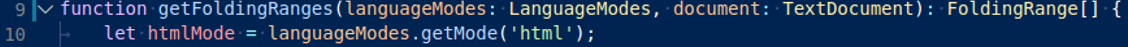
\includegraphics[width=10cm]{assets/figures/semantic-coloration-with.png}
    \end{center}
    \caption[Avec coloration sémantique ]{\label{semantic-coloration-with} Avec coloration sémantique }
\end{figure}

\begin{figure}[!ht]
    \begin{center}
        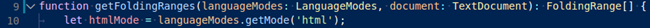
\includegraphics[width=10cm]{assets/figures/semantic-coloration-without.png}
    \end{center}
    \caption[Sans coloration sémantique]{\label{semantic-coloration-without} Sans coloration sémantique}
\end{figure}

On voit à la ligne 10 que la colorisation de la fonction a changé et correspond maintenant à un paramètre d'une fonction.
Cela est donc intéressant pour des langages plus complexes dans leur nature qu'un langage de sérialisation. Une coloration syntaxe suffit amplement dans notre cas.
Car se baser sur la structure du document nous donne déjà toutes les informations nécessaires.

\section{Auto-completion}
Cette fonctionnalité fait parti de ce qu'on appelle plus communément \href{https://code.visualstudio.com/docs/editor/intellisense}{"IntelliSense"} qui un terme général désignant diverses fonctions d'édition de code.

Comme mentionné au début de ce document, une approche typique pour implémenter de la complétion est d'utiliser directement un parser du langage.

Mais en complément nous allons utiliser en plus "Antlr4-c3" (Code Completion Core for Antlr4, aussi simplement nommé c3).

Il s'agit d'un moteur de complétion pour les parsers basés sur ANTL4. Le moteur c3 est capable de fournir des candidats de complétions.

Avant il n'y a avait que des solutions customs. Cette librairie a pour objectif de fournir une implémentation commune. Il est disponible comme node module et est écrit en Typescript.

Nous utilisons la version 4 de ANTLR. Elle a comme avantage sur son ancienne version (ANTL3) d'avoir la strucuture de la grammaire directement disponible dans le parser via
un mécanisme de machine à état ATN (Augmented Transition Network). C'est ce méchanisme qui est en coeur du fonctionnement du moteur.

Dans la configuration la plus simple pour l'utiliser, il suffit de lui donner une instance du parser et une position de caret (notre curseur) pour qu'il renvoie les candidats correspondants.
Cette position est l'indice du candidats. L'explication pour le trouver ce trouve dans la séction \hyperref[candidates]{\textbf{Candidats}}

On constate donc que c'est un outil relativement puissant et qui nous simplifie grandement la tâche.

\textbf{Remarque}: On pourrait penser qu'avoir à disposition un parser nous permettrait de récupérer toutes les informations nécessaires au travers d'un AST. Cependant ce n'est pas le cas pour la plupart des scénarios.
Nous pouvons savoir quels sont les tokens valide à un emplacement (ce qui est suffisant pour nous). Mais pour certains langages, des informations manquent. Par exemple des noms de classe, des objets de base de données, des membres de classes, des fonctions, etc. ne sont pas représentés dans la grammaire. 

Ci-dessous Un ATN d'une séquence :

\begin{figure}[!ht]
    \begin{center}
        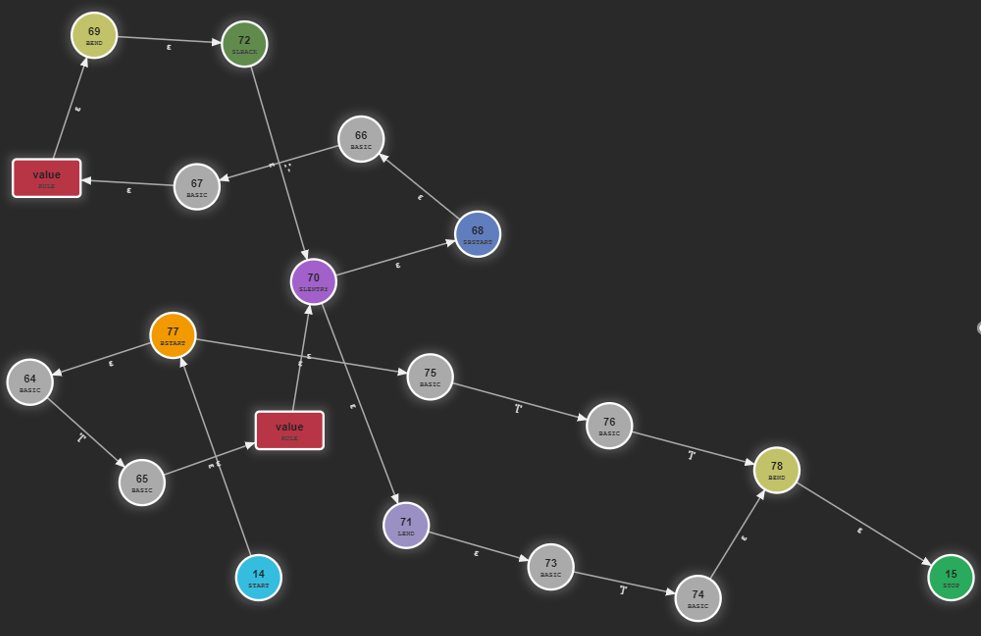
\includegraphics[width=10cm]{assets/figures/seq_ATN.png}
    \end{center}
    \caption[ATN d'une séquence]{\label{seq_ATN} ATN d'une séquence}
\end{figure}

La seule contrainte est qu'il est nécessaire que tout le code se trouvant avant le curseur soit correct. Mais ce qui se trouve à la suite peut être erroné.
Ainsi, nous pouvons revenir n'importe où dans le code, car la partie se trouvant après le curseur n'est pas prise en compte et la rédaction du code précédente est normalement correcte.
De plus, actuellement, nous n'avons pas de suggestions qui dépendrais de ce qui se trouve après le curseur.
Car par exemple dans l'exemple suivant pour du code SQL :

\begin{lstlisting}
SELECT | FROM USER // ("|" étant le curseur)
\end{lstlisting}

Dans ce scénario des suggestions liées à la table USER devrait être proposé et donc un traitement particulier devrait être fait.
La seule chose qui doit donc être correcte est la structure du code. C'est-à-dire que l'ordre des éléments attendus est respecté.

\subsection{Tolérance}
Il semble normal que la complétion n'ait pas lieu si le code saisie est gravement erroné.
Cependant il devrait être tolérent à une certain mesure sur des erreurs qui ne péjore pas la compréhension du code.
Une possiblité et de traiter les erreurs lors de l'analyse syntaxique, ce sujet est abordé dans la section \hyperref[error handle]{Gestion des erreurs} ci-dessous.

Mais on peut imaginer supprimer des cas potentiels d'erreurs lors de la conception de notre grammaire.
Par exemple, les erreurs sur les valeurs attendues. Une stratégie serait d'avoir un type seul qui supporterait le plus de symboles possibles.
Imaginons que l'on donnerait en entré un type incorrect à une propriété, selon la spécification officielle du langage UON.
Par exemple (max : 12a), l'erreur pourrait tout simplement ne pas exister.
Ainsi même si cela est faux syntaxiquement en UON, cela ne bloque pas le processus de l'auto-complétion.

Pour signaler à l'utilisateur que la saisie est tout de même incorrect. On peut s'aider en parallele de la coloration syntaxique.

\subsection{Mécanisme automatique}
VsCode va automatiquement filtrer les suggestions pendant la saisie.
Par défaut il propose également des symboles déjà existants dans le code dans ses suggestions.

\subsection{Gestion des erreurs}\label{error handle}
On peut ajouter au parser un "ErrorListener".
Par défaut c'est la stratégie de la classe se trouvant dans le fichier \href{https://github.com/tunnelvisionlabs/antlr4ts/blob/master/src/DefaultErrorStrategy.ts}{suivant} qui est appliquée.

Mais on peut l'étendre pour redéfinir les fonctions.
Car normalement en cas d'erreur, le parser va essayé de continuer le parsing jusqu'à trouver un token valide.
Cependant comme il se peut qu'il n'y ait rien après. C'est presque tout le temps le cas lorsqu'on est en train d'écire.
On va donc juste s'arrêter.

\subsection{Snippets}
Il est possible d'ajouter des snippets sous Vscode. C'est-à-dire des templates qui nous permettent de générer du code prédéfini. Puis de les ajouter aux suggestions.
C'est utile si à un moment donné on a le choix entre plusieurs suggestions et que l'on veut tous les avoir d'un coup.
Par exemple, on peut en UON, ajouter des attributs à un schéma :

\begin{figure}[!ht]
    \begin{center}
        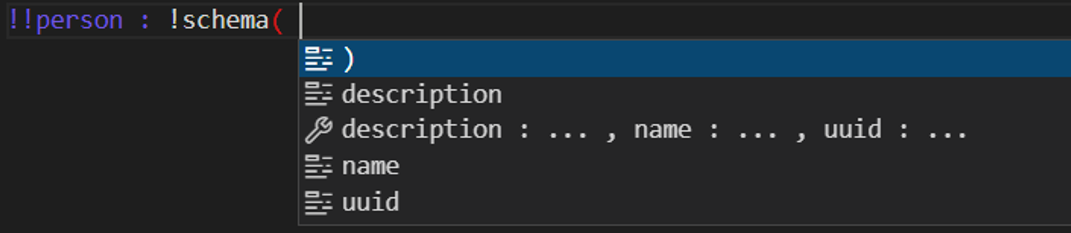
\includegraphics[width=10cm]{assets/figures/snippet-suggestion.png}
    \end{center}
    \caption[Suggestion d'un snippet]{\label{snippet-suggestion} Suggestion d'un snippet}
\end{figure}

Cependant toute la difficulté et de proposer ces suggestions au bon moment, car ne faisant pas partie du moteur de complétions d'antlr. Une idée et de se baser sur le dernier token reconnu. On pourrait ici savoir qu'il est le moment d'ajouter ce snippet, si le dernier token est de type "!schema".

\subsection{Triggers}
L'éditeur va trigger automatiquement l'autocomplétions en appelant le provider lorsque l'on saisit plusieurs caractères. Il aussi possible de l'activer manuellement en exécutant la commande "ctr + space".
On peut aussi ajouter au provider des symboles qui vont trigger son activation. Les symboles espace et de retour à la ligne ont été défini comme triggers, car cela semble assez naturel dans ce langage. Cependant il ne s'agit seulement d'une appréciation personnelle.

\subsection{Candidats}\label{candidates}

Actuellement pour connaitre l'indice du ou des prochains candidats, on récupère le flux des tokens (tokenStream) trouvé lors du parsing.
Puis, on récupère dans un tableau chaque token individuellement (y compris les espaces).

Cependant lorsque l'utilisateur écrit et que cela trigger l'autocomplétion, le texte parsé est souvent inccorect, car le dernier élément saisi n'est pas encore complet.

Grâce à la taille du tableau et en se basant sur les erreurs qui ont été généré, on peut déduire l'indice du ou des prochains tokens que l'on peut afficher.

\subsubsection{Index du candidat}
L'indexation est gérée de 2 manières différentes. En fonction de la prise en compte de l'espace ou non.

\begin{figure}[!ht]
    \begin{center}
        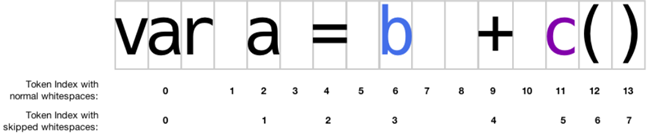
\includegraphics[width=10cm]{assets/figures/candidat-index.png}
    \end{center}
    \caption[Indexation des candidats]{\label{candidat-index} Indexation des candidats}
\end{figure}

Cela va dépendre si on décide d'ignorer ou non les espaces dans la grammaire g4.
Les dévelopeurs de c3 recommandent de pas ignorer les espaces. Car cela permet de gérer plus de cas particuliers.

\section{Document outlining}
\textbf{[TODO]}

\section{Info on Hover}
\textbf{[TODO]}

\section{Fonctionnalités triviales}
Il s'agit de fonctionnalités couramment disponibles dans un support de langage. Leur implémentation est relativement simple et rapide et n'a donc pas été mentionnée dans le cahier des charges.

Les suivantes ont été implémentées :
\textbf{Comment}
\begin{itemize}
    \item Il est possible de commenter du code sous forme de ligne.
    \item Il est possible de commenter et décommenter du code (Toggling)
\end{itemize}

\textbf{Symbol pairs}
\begin{itemize}
    \item Il est possible de faire la correspondance pour certaines paires de symboles à l'aide d'une indication visuelle. (Matching)
    \item Certains symboles du langage doivent être automatiquement complétés si l'utilisateur saisit le premier élément de celle-ci. (Autoclosing)
\end{itemize}

\textbf{Code folding}
\begin{itemize}
    \item Cacher un bloc de code sur une ligne en fonction de son niveau d'indentation.
\end{itemize}

Pour pouvoir les implémenter, il suffit d'éditer un fichier de configuration json (language-configuration.json) puis  éditer le fichier package.json afin qu'il référence ce fichier sous le point "contribution".

\chapter{Intégration continue}

\section{Autocomplétion}
Applique la même méthodologie de antlr4-ts : \href{https://github.com/mike-lischke/antlr4-c3/tree/master/test}{https://github.com/mike-lischke/antlr4-c3/tree/master/test}
\textbf{[TODO]}

\section{Syntax highlight}
\textbf{[TODO]}

\section{Outline view}
Teste que l'arbre syntaxique reçu est celui attendu pour un code.
\textbf{[TODO]}

\section{Information Hover}
Tester que l'élément on Hover soit celui attendu
\textbf{[TODO]}

\chapter{Conclusion}
\textbf{[TODO]}

%% \vfil
%% \hspace{8cm}\makeatletter\@author\makeatother\par
%% \hspace{8cm}\begin{minipage}{5cm}
%%if
% Place pour signature numérique
%%\printsignature
%%fi
%% \end{minipage}
%% \clearpage

%% \let\cleardoublepage\clearpage
%% \backmatter

%% \label{glossaire}
%% \printnoidxglossary
\printbibliography
\addcontentsline{toc}{chapter}{Bibliographie}
%% \label{index}
%% \printindex

\end{document}
